\chapter{Design and Implementation} \label{ch:proposal}

\section{Preprocessing}

First, the signal is fixed for DC offset by subtracting the mean sample value, and normalized to a prechosen threshold. Then we trim the signals using the algorithm described in \cite{6778857}.

The trimming algorithm uses short-time energy and zero crossing rates and it possesses a self-adapting nature towards the background acoustic environment. The energy is given by sum of magnitudes of samples near the window,
\begin{equation} E(n) = \sum_w|s(n+i)| \end{equation}

The threshold variables can be calculated as given in following equations \cite{6778857}.

\begin{equation} I1 = 0.03 \times (IMX - IMN) + IMN \end{equation}
\begin{equation} ITL = MIN(I1 , 4 \times IMN), ITU = 5 \times ITL \end{equation}
    
\begin{figure}[h!]
    \centering
    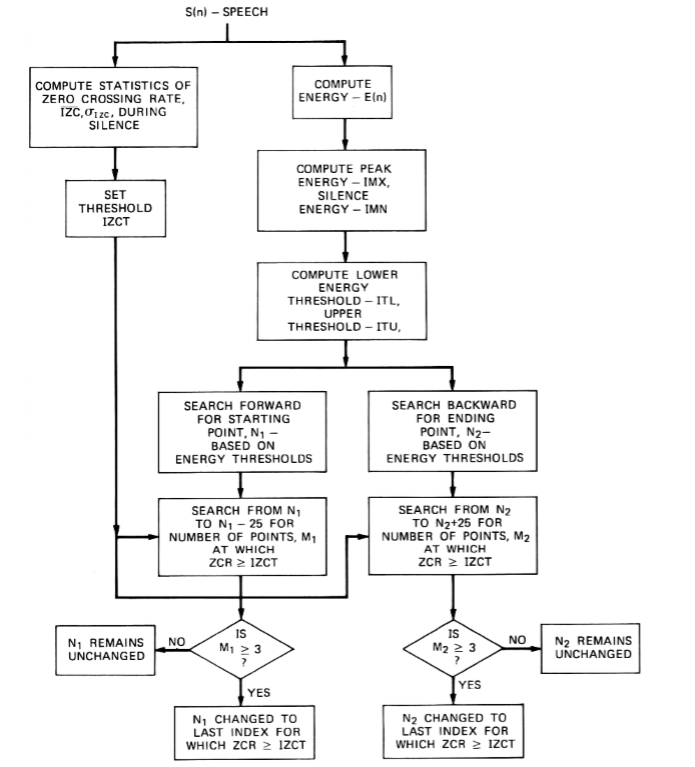
\includegraphics[scale=1.0]{trim-algo-flowchart}
    \label{fig:trim-algo-flowchart}
    \caption{Trimming algorithm flowchart \cite{6778857}}
\end{figure}

\section{Phoneme Segmentation using Pitch Period Analysis}

A speech signal can be classified into voiced, unvoiced and silence regions. There is no excitation during the silence region and majority of speech regions including vowels and semi vowels are voiced. We use \cite{1162765} to label the segments as voiced or unvoiced and then find their boundaries.

\begin{itemize}
\item Find peak signal threshold from the beginning background noise.
\item Select segments of length 300 samples with a moving window of 100 samples.
\item The segment is silence if peak signal level is below threshold.
\item Find clipping level as a fixed percentage of the minimum of the maximum absolute values in the first and last 100 samples of segment.
\item Clip the signal and then compute the autocorrelation function.
\item Compare peak of autocorrelation function with the fixed threshold and classify the segment as unvoiced if the peak falls below, and as voiced if above.
\end{itemize}

\section{Linear Predictive Coding Feature Extraction}

Linear Predictive Coding is very useful for encoding high quality speech at a low bit rate and provides extremely accurate estimates of speech parameters. Its main advantage comes from the reference to a simplified vocal tract model and the analogy of a source-filter model with the speech production system.

After cutting the phonetic units, we find out the linear predictive cepstral coefficients(LPCC) using the autocorrelation method from \cite{rabinerbook}. First, the phoneme is divided into overlapping segments, and then we apply a tapering window to each segment to hide the discontinuities.

\subsubsection{Autocorrelation Analysis}

The next step is to find the autocorrelation for each frame of windowed signal with

\begin{equation} \sum_{n=0}^{n-1-m}{\tilde{x}_l(n)}{\tilde{x}_l(n+m)}, \quad \begin{aligned} m=0,1,...,p. \end{aligned} \end{equation} 

\subsubsection{LPC Analysis}
The p + 1 autocorrelations are mutated to LPC coefficients by using Durbin’s method:
\begin{equation} E^{(0)} = R(0) \end{equation}
\begin{equation} k_i = \dfrac{R(i) - \sum_{j=1}^{i-1}\alpha_j^{i-1}R(|i-j|)}{E^{i-1}},  \quad \begin{aligned} 1 \leq i \leq p. \end{aligned} \end{equation}
\begin{equation} \alpha_i^{(i)} = k_i \end{equation}
\begin{equation}\alpha_j^{(i)} = \alpha_i^{(i-1)} - k_i\alpha_{i-1}^{(i-1)},   \quad \begin{aligned} 1 \leq j \leq i-1. \end{aligned}\end{equation}
\begin{equation} E^{i} = (1-k_i^2)E^{i-1} \end{equation}

In the last step, the LPC cepstral coefficients are derived from the LPC coefficients. A sine window is applied over the cepstral coefficients to desensitize them towards noise and noise like sounds. 

\begin{figure}[h!]
    \centering
    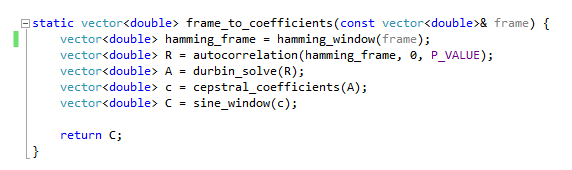
\includegraphics[scale=1]{lpc-code}
    \label{fig:lpc-code}
    \caption{Linear predictive coding implementation}
\end{figure}

\begin{figure}[h!]
    \centering
    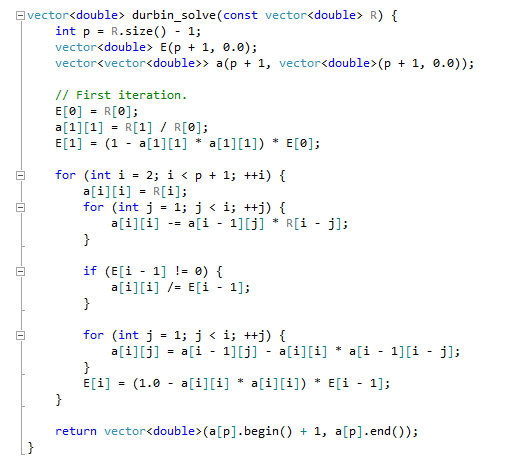
\includegraphics[scale=1]{durbin-code}
    \label{fig:durbin-code}
    \caption{Durbin solve implementation}
\end{figure}


\section{Template Matching}

We use Tohkura Distance for finding the distance between coefficients. The measure is a statistically weighted distance measure with weights equal to the inverse variance of the cepstral coefficients \cite{1165058}.

The coefficients are the templates for recognising digits. We generate the training coefficients for each phoneme in each utterance. When we get the test signal, we apply the same preprocessing and feature extraction to get the test coefficients for each phoneme of the test signal. Then for each phoneme unit from test signal, we find its distance with respect to each phoneme unit in our training data using their coefficients. We output the digit, which gives the least average distance for all its phonemes.